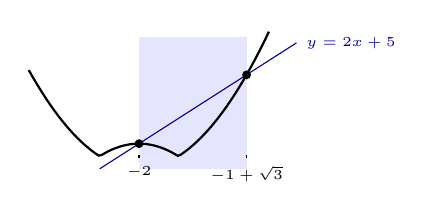
\begin{tikzpicture}[x=5mm,y=1.6mm]
\fill[blue!10] (-2,-1) rectangle (0.732,9.5);
\ax{-5}{2}{-1}{9.5}
\draw[thick,domain=-4.8:1.3,samples=80] plot (\x,{abs((\x)^2+4*\x+3)});
\draw[blue!60!black,domain=-3:2,samples=80] plot (\x,{2*\x+5});
\draw (-2,0.12)--(-2,-0.12); \node[below] at (-2,0){\tiny $-2$};
\draw (0.732,0.12)--(0.732,-0.12); \node[below] at (0.732,0){\tiny $-1+\sqrt3$};
\fill (-2,1) circle (1.6pt);
\fill (0.732,6.46) circle (1.6pt);
\node[blue!60!black,right] at (2,9){\tiny $y=2x+5$};
\end{tikzpicture}